\section{Project Planning}
A good amount of planning to make sure the group has been well organized were invested early in the project. In this section the planning phase will be presented. An evaluation of how this worked out over the course of the project can be found in chapter \ref{evaluation} Evaluation.

 
\subsection{Group organization}
The group has consisted of five Computer Science students, all finishing their third year at NTNU.

At an early stage in the project, the group decided to not assign strict areas of responsibility, apart from the Scrum-master position. The reason behind this is the nature of the project task. A lot of research needed to be done before getting a good overview of the task, and how extensive each part was. Giving narrow areas of responsibility therefore seemed unnecessary. However, a rough outline of main areas of responsibility were set. Below follows a brief presentation of each group member and their responsibilities.
\\

\noindent \textbf{Rikard Eide} \\
Scrum-master. Rikard has previously worked three years part time at a hospital. Based on this experience he was given the main responsibility with researching the industry. He has experience with Java, and is familiar with C\# and .Net.
\\

\noindent \textbf{Magnus Lund} \\
Magnus has experience with Java, \LaTeX\ and has worked on a couple of smaller Android projects. His main responsibility was managing the code- and application parts of the project.
\\

\noindent \textbf{Jens Kristian Espevik} \\
Jens Kristian's main responsibility, aside from coding, has been with group formalities, such as constructing meeting notes, weekly updates and report writing.
\\

\newpage

\noindent \textbf{Andreas Røyrvik} \\
Andreas has experience with server management and back-end development, and this has been his main responsibility.
\\

\noindent \textbf{Joakim Pettersen} \\
Joakim has experience with Java and Android. Joakim's main responsibility was testing.
\\


\subsection{Project management tools}
\label{project_management_tools}
To administrate the sprints and project organization in general, it was together with the customer, decided to use Confluence \cite{confluence} and JIRA Agile \cite{jira}. These are common tools in the industry which the group was recommended to use. The customer had access to both of these tools, and could follow the progress closely.

\subsubsection{Confluence}
Confluence is a team collaboration tool. Necessary diagrams and figures were developed with plugins found in the system. Other documentation, such as user manuals, technical descriptions and various tables were created, maintained and stored in Confluence. Confluence is used to ensure that the documentation is stored in such a way that it is easy to navigate and update if needed.

\subsubsection{JIRA Agile}
JIRA Agile is an issue tracker used to track, assign and report work tasks. JIRA helped the group visualize remaining tasks in each sprint as well as providing tools for generating progress reports based on task completion.


\subsection{Communication}
To communicate on a daily basis, the group used Google+'s Hangouts and Groups \cite{hangouts}. In addition to traditional real time text based chat, Google Hangouts offers video and voice chat. This turned out to be an useful feature when doing daily Scrum stand-ups on days where no in-person meetings were held.

To communicate with the customer and the supervisor, traditional email was used. In addition to communication over email, the group had bi-weekly meetings with the supervisor and customer.

\subsection{Work breakdown}
\label{workbreakdown}

The group did not receive any formal requirements from the customer. To get a better understanding of the customer's idea of the application built, frequent meetings were arranged in the beginning of the project period. To prepare for these customer meetings, the group had frequent internal meetings as well. In these meetings we discussed our initial impression of the application idea, and our thoughts about requirements. It was decided that each group member was to create several user stories, and present them to the group. A compilation of what we though would be the most relevant user stories were put together and presented to the customer.

The group also tried to identify what was the major work areas of the project, such as GUI implementation, image handling, user authentication etc. To help decide how extensive these tasks were, the group used Scrum poker cards to assign a weighted value to these areas of development.

This eventually lead to the creation of \emph{epics}. In agile development an epic is a compiled set of user stories describing a major product feature. The group then used the estimates to assign these epics to specific sprints, as seen in Figure \ref{fig:sprinter_oversikt}. Because we recognized this project would depend on research and information not yet obtained, traditional planning tools like Gantt and work-break-down charts were deemed ineffective. The group attempted to design the epics to be as independent of each other as possible, to allow for implementation of them in any order. The sprints were assigned ''code-names'', making it easier to distinguish between them. A discussion on how this process panned out during the project, can be found in section \ref{researchEval}.


\begin{figure}[H]
\centering
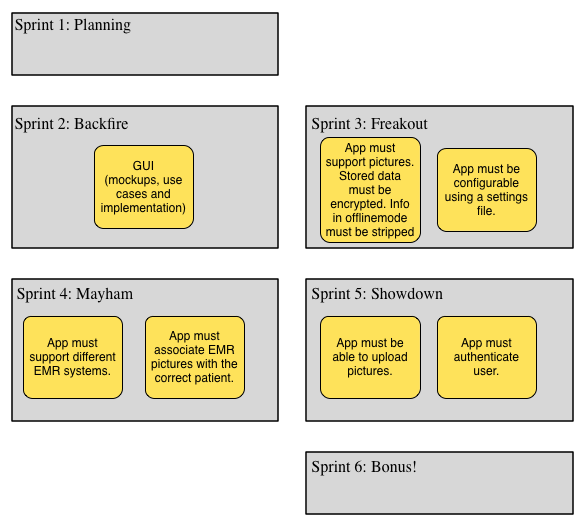
\includegraphics[scale=0.7]{img/sprint_overview.png}
\caption{Overview of the sprints and their goals}
\label{fig:sprinter_oversikt}
\end{figure}


\subsection{Work methodology}
Having some experience with Scrum, the group decided to go for an agile Scrum methodology. The focus was on frequent communication with the customer, use of agile collaboration software (see section \ref{project_management_tools}) and typical agile development practices like daily stand-ups. In this section, various agile concepts and how we used them in the project will be presented.


\subsubsection{Product backlog}
At the highest level, this is a set of stories describing the different functions of the system. These stories were broken up to a list of smaller, concrete issues. The customer had access to this list, and was able to add and subtract functionality as the product evolves.


\subsubsection{Planning and effort estimation}
With the product backlog as the basis, each task was estimated. The estimate represented how many hours we though were needed to complete a given task. This was initially meant to be re-done at the start of every sprint. However, due to the amount of research needed to be done throughout the project and the uncertainty about the extent of each task before we got in touch with the right experts, we abandoned this idea after the first sprint. The estimates were so far off they served no purpose.


\subsubsection{Sprint backlog}
Tasks were be estimated, prioritized and put into a \emph{backlog} containing all available tasks for the given sprint. Because the group was not given a requirements document in the beginning of the project, additional tasks were often added continuously in the sprint backlog when research revealed new requirements.


\subsubsection{Daily stand-up and work sessions}
Daily \emph{stand-ups} were arranged Monday through Friday. A stand-up meeting is a short meeting with all the team members where the purpose is to update each other on the project status and individual progress. Lasting no more than a total of 5-15 minutes, each team member should answer the following questions:
\begin{itemize}
     \item \emph{What have I done since the last meeting?}
     \item \emph{What will I do today?}
     \item \emph{Did I encounter any problems hindering my progress?}
\end{itemize}
\noindent
The group had mandatory work sessions at campus three times a week.


\subsubsection{Sprint end and demo}
At the end of each sprint, a few of the group members met with the customer and demonstrated a working version of the product. This opportunity was also used to discuss the backlog. Getting direct feedback from the customer could help point us in the right direction.
%It was also very helpful for us to get direct feedback while demonstrating the application at its current state.


\subsubsection{Sprint retrospective}
After each sprint, the team got together and looked at the past two weeks. Two key points were discussed in these meetings:

\begin{itemize}
     \item What went good?
     \item What went bad and/or should have been done different?
\end{itemize}
\noindent
It is important to identify both positive and negative parts about the sprints while they are still fresh in memory. That way the group knew what to focus on improving in the next sprint, and what to continue doing.

Based on experiences from the sprint retrospective meeting and feedback from the sprint end demo, the product backlog was re-evaluated.


\subsection{Milestones}
At the beginning of the project the group created milestones based on the limited information available. How these milestones were planned according to the sprints can be seen on the next page.

\begin{table}[H]
\begin{tabular}{p{2cm}p{11cm}}
%09.02.2014 & \emph{Preliminary version of the report:} A brief overview of work done up to this point, focusing on planning and organization. \\
14.02.2014 & \emph{Sprint 1 end:} Sprint end. \textbf{Milestone:} Ready to code. At this point the implementation can start. \\
28.02.2014 & \emph{Sprint 2 end:} Sprint end and product demonstration for the customer. \textbf{Milestone:} GUI ready for implementation. The plan for the GUI is ready and the usability test is done. \\
14.03.2014 & \emph{Sprint 3 end:} Sprint end and product demonstration for the customer. \\
%16.03.2014 & \emph{Mid-semester version of the report:} A more detailed overview of work done up to this point. Should contain an architecture and a plan for how to meet the requirements set. \\
28.03.2014 & \emph{Sprint 4 end:} Sprint end and product demonstration for the customer. \\
11.04.2014 & \emph{Sprint 5 end:} Sprint end and product demonstration for the customer. \textbf{Milestone:} Potentially shippable product \\
02.05.2014 & \emph{Sprint 6 end:} Sprint end and product demonstration for the customer. \textbf{Milestone:} Code freeze \\
%30.05.2014 & \emph{Final version of the report:} Deliver the complete report. \\
02.06.2014 & \emph{Product demo for the customer:} Demonstration of the final application for the customer. \\
\end{tabular}
\end{table}



\subsection{Risk management}
As suggested early on by the group's supervisor, getting a risk management plan ready was prioritized. A list of risks that could possibly threaten the project were set up. Having a plan is important to better tackle any problems should they arise. It is also a preventive measure, because it spreads awareness of potential problems to look out for. Risks have various consequences and potential impact on progress. Some are unavoidable and out of our hands, while others should be avoided at all cost. An example of the former is illness within the group. Risks are a product of two parameters: the probability of the loss happening and the consequence should the loss occur. A detailed description of identified risks can be found in Appendix \ref{risk}.
